\documentclass{beamer}
\usepackage[utf8]{inputenc}
\usepackage{graphicx}
\usepackage{svg}
\usetheme{Goettingen}

\title{Segurança em redes}
\subtitle{exemplos de exploits comuns e como lidar com elas}
\author{Giuliano Oliveira de Macedo}
\institute{}
\date{}

\begin{document}

\begin{frame}
\titlepage 
\end{frame}

\section{Importância de segurança em redes}

\begin{frame}
\frametitle{Modelo de software TCP/IP }
\begin{figure}[htp]
	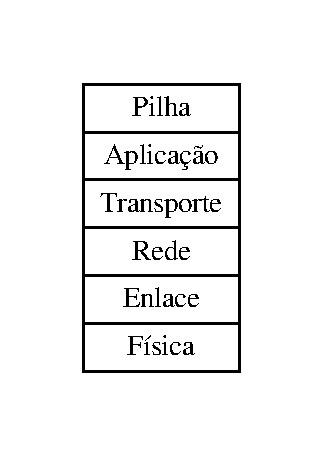
\includegraphics[width=6cm]{pilha1.pdf}
\end{figure}

\end{frame}

\begin{frame}
\frametitle{Modelo de software TCP/IP }
\begin{figure}[htp]
	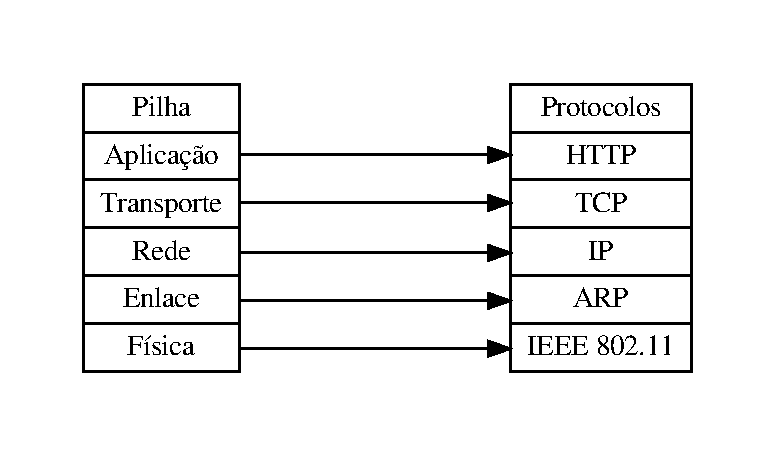
\includegraphics[width=10cm]{pilha2.pdf}
\end{figure}

\end{frame}

\begin{frame}
\frametitle{Modelo de software TCP/IP }
\begin{figure}[htp]
	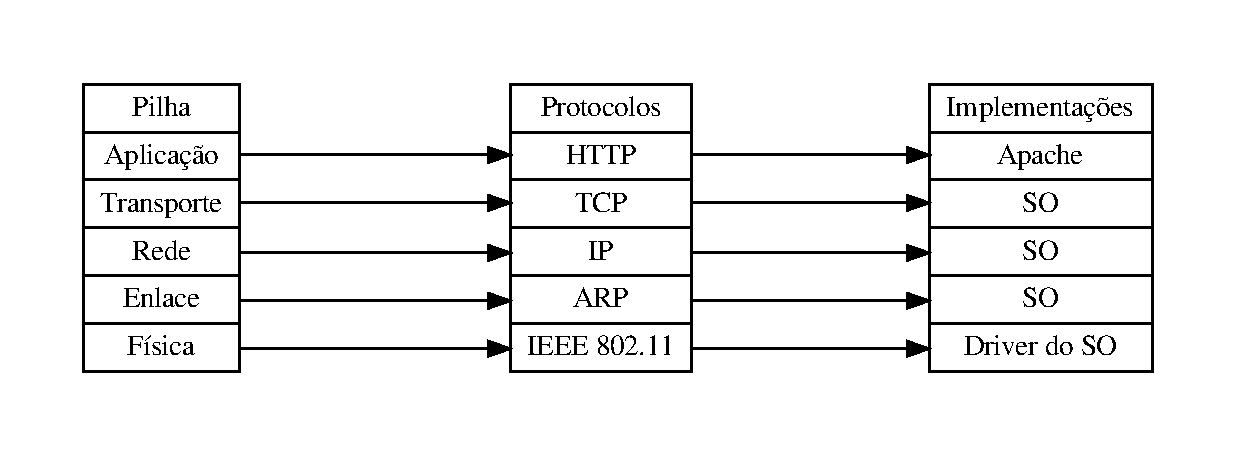
\includegraphics[width=10cm]{pilha3.pdf}
\end{figure}
\end{frame}

\section{Contextualização}
\begin{frame}
	\frametitle{CVE}
	\begin{figure}[htp]
		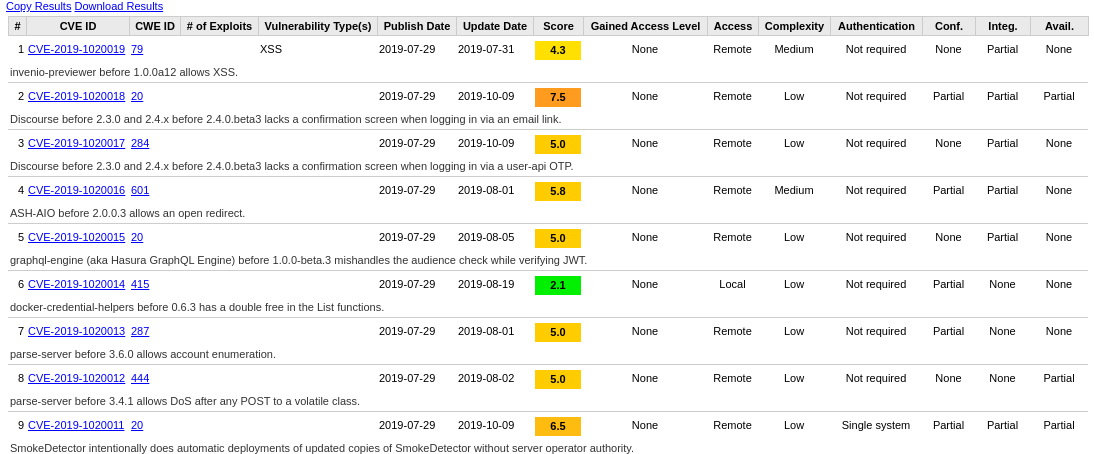
\includegraphics[width=9cm]{cve.png}
	\end{figure}
\end{frame}

\begin{frame}
	\frametitle{Termos comuns}
	
	\begin{itemize}
		\item Vulnerabilidade
		\begin{itemize}
			\item Qualquer falha ou brecha no algoritmo
		\end{itemize}
		\item Exploit
		\begin{itemize}
			\item Implementação real de uma vulnerabilidade
		\end{itemize}
		\item Exemplo de vulnerabilidades
		\begin{itemize}
			\item Buffer overlfow
			\item DoS
			\item Execução de código
			\item Sql Injection
			\item XSS
			\item Bypassing
			\item Ganhar informações
			\item Elevar privilégio
			\item etc
		\end{itemize}
	\end{itemize}
\end{frame}
\begin{frame}
	\frametitle{Ataques comuns ao longo dos anos 1999-2019}
	\begin{figure}[htp]
			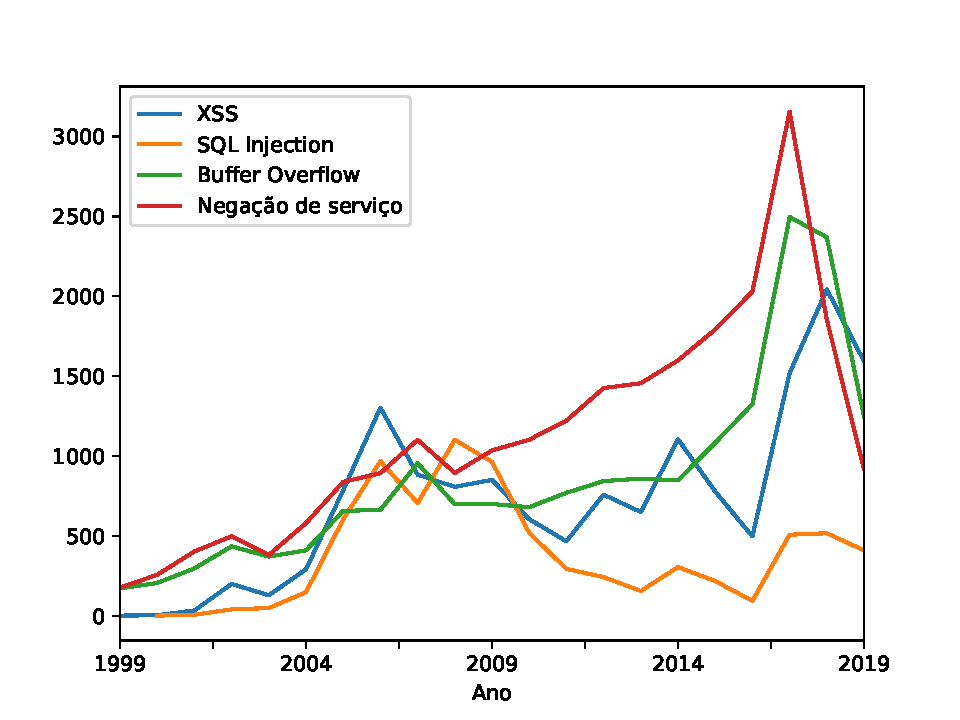
\includegraphics[width=10cm]{no_ataques.pdf}
		\end{figure}
\end{frame}

\section{Ataques}
\begin{frame}
	\frametitle{Exemplos de ataques e correspondência com o modelo de redes de 5 camadas}
	\begin{figure}[htp]
		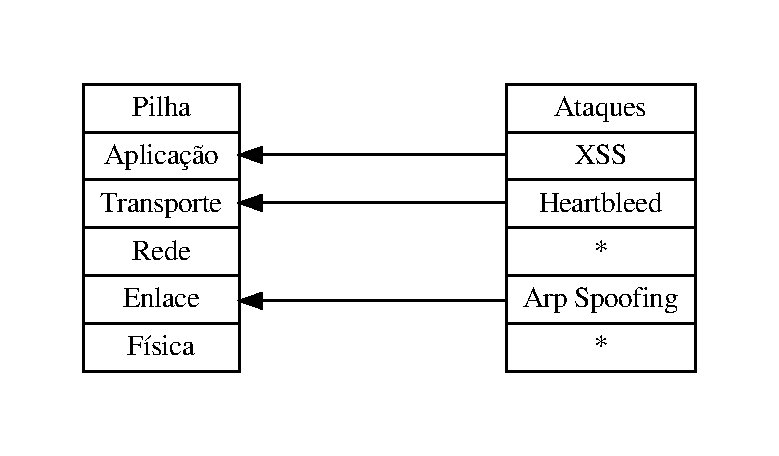
\includegraphics[width=8cm]{pilha_ataque.pdf}
	\end{figure}
\end{frame}
\begin{frame}
	\frametitle{Exploits que irei mostrar}
	\begin{itemize}
		\item XSS (Cross server scripting)
		\item ARP Spoofing (Manipulação de servidores/clientes ARP com o fim de espionagem)
	\end{itemize}
\end{frame}

\subsection{XSS}
\begin{frame}
	\frametitle{Exemplo}
\end{frame}

\begin{frame}
	\frametitle{Mitigação}
	Problemas:
	\begin{enumerate}
		\item O usuário deve ter o poder de ainda estilizar o texto
		\item Tags de injeção de JS devem ser ignoradas
	\end{enumerate}
\end{frame}

\begin{frame}
	\frametitle{Minha solução}
	Solução para o problema 1\\
	(O usuário deve ter o poder de ainda estilizar o texto)\\
	Usar outra linguagem de marcação de texto como o \textbf{Markdown}
	\begin{figure}[htp]
		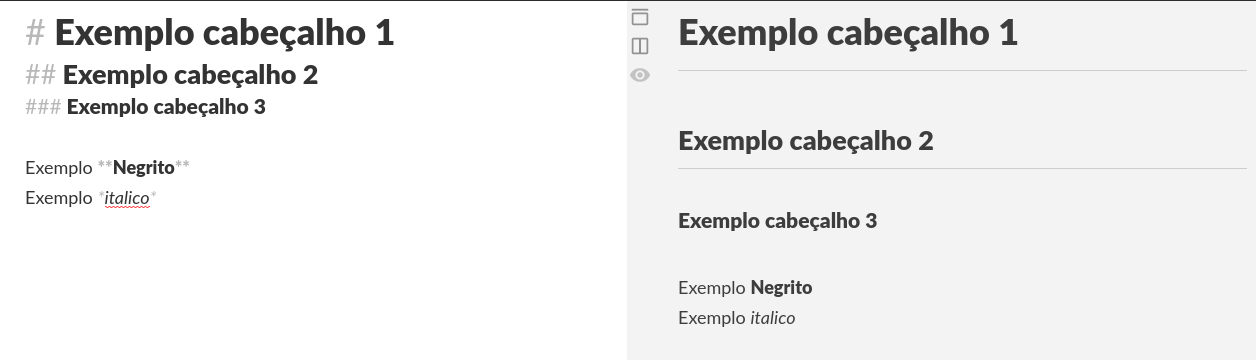
\includegraphics[width=10cm]{markdown_example.png}
	\end{figure}

\end{frame}

\begin{frame}
	\frametitle{Minha solução}
	Solução para o problema 2\\
	(Tags de injeção de JS devem ser ignoradas)\\
	Limitar o alfabeto do usuário:
	\textbf{Apenas os caracteres alfanuméricos com acento, números, os caracteres \# e * serão aceitos}

\end{frame}

\subsection{ARP Spoofing}
\begin{frame}
\frametitle{Exemplo}
\begin{figure}[htp]
		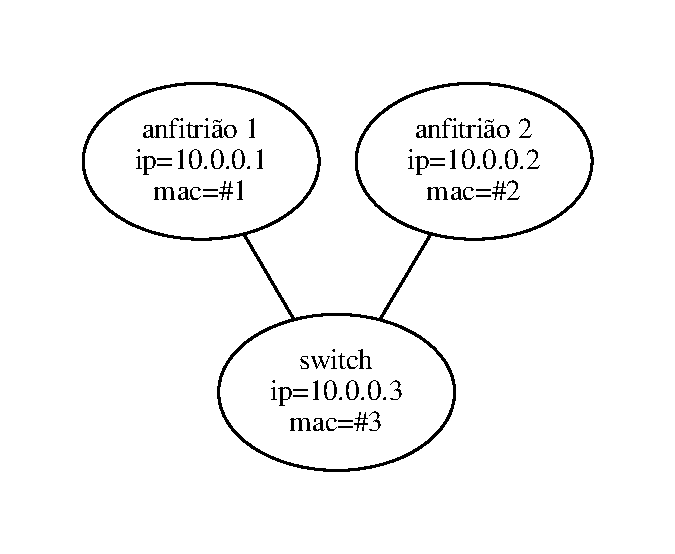
\includegraphics[width=10cm]{topo.pdf}
	\end{figure}
\end{frame}

\begin{frame}
\frametitle{ARP Spoofing}
	site HTTP não seguro de propósito:
	\url{http://testing-ground.scraping.pro/login}
\end{frame}

\begin{frame}
\frametitle{Mitigação}
	Softwares de defesa :
	\begin{itemize}
		\item Agnitum Outpost Firewall
		\item AntiARP
		\item Antidote
		\item Arp\_Antidote
		\item Arpalert
		\item Etc
	\end{itemize}
	Outra solução\\
	\textbf{HTTPS}
\end{frame}

\section{Referências}
\begin{frame}
	\frametitle{Referências}
	\bibliographystyle{amsalpha}
	\bibliography{references.bib}
	\nocite{*}
\end{frame}

\begin{frame}
	\frametitle{Obrigado}
	Código fonte dos exploits e desse slide estão disponíveis no repositório github:\\ \url{https://github.com/llpinokio/rc2t2}
\end{frame}


\end{document}